\documentclass[UTF8]{ctexart}
\usepackage{graphicx}
\usepackage{ctex}
\usepackage{tikz}
\usepackage{amsmath}
\title{热力学与统计物理-第七次作业}
\author{吴远清-2018300001031}

\begin{document}
    \maketitle
    Problem 5.11\\
    Answer:\\
    Let's the solid expands an increment of $dV$, we have:
    $$V + dV = (x+dx)(y+dy)(z+dz) \eqno(1.1)$$
    Ignore the orders that higher than 1:
    $$V + dV = V + yzdx + xzdy + xydz \eqno(1.2)$$
    So:
    $$\alpha = \frac{1}{V}\frac{dV}{dT} = \frac{1}{x}\frac{dx}{dT} + \frac{1}{y}\frac{dy}{dT} + \frac{1}{z}\frac{dz}{dT} = 3\alpha_L \eqno(1.3)$$

    Problem 5.13\\
    Answer:\\
    From the first law:
    $$C_p = T(\frac{\partial s}{\partial T})_p \eqno(2.1)$$
    $$(\frac{\partial C_p}{\partial p})_T = T(\frac{\partial}{\partial p})_T(\frac{\partial s}{\partial T})_p = T(\frac{\partial}{\partial T})_p(\frac{\partial s}{\partial p})_T \eqno(2.2)$$
    From the Maxwell relation and the definition of $\alpha$:
    $$(\frac{\partial C_p}{\partial p})_T = \alpha^2vT - vT\frac{d\alpha}{dT} \eqno(2.3)$$

    Problem 5.14\\
    Answer:\\
    (a):\\
    $$TdS = dE - FdL \eqno(3.1)$$
    (b):\\
    From (3.1) we may read off the Maxwell relation:
    $$\left(\frac{\partial S}{\partial L}\right)_{T}=-\left(\frac{\partial R}{\partial T}\right)_{L} \eqno(3.2)$$
    Since:
    $$F = aT^2(L-L_o) \eqno(3.3)$$
    So:
    $$\left(\frac{\partial S}{\partial L}\right)_{T}=-2 a T\left(L-L_{O}\right) \eqno(3.4)$$
    (c):\\
    $$s\left(L_{0}, T\right)-S\left(L_{0}, T_{0}\right)=\int_{T_{0}}^{T} \frac{C_{L}}{T^{\prime}} d T^{\prime}=\int_{T_{0}}^{T} \frac{b T^{\prime}}{T^{\prime}} d T^{\prime}=b\left(T-T_{0}\right) \eqno(3.5)$$
    $$S(L, T)-S\left(L_{0}, T\right)=\int_{I_{0}}^{L}\left(\frac{\partial S}{\partial L}\right)_{T} d L=\int_{L_{0}}^{L}-2 a T\left(L^{\prime}-L_{0}\right) d L^{\prime}=-a T\left(L-L_{0}\right)^{2} \eqno(3.6)$$
    So:
    $$S(L, T)=S\left(L_{0}, T_{0}\right)+b\left(T-T_{0}\right)-a T\left(L-L_{0}\right)^{2} \eqno(3.7)$$
    (d):\\
    In this process which $\Delta S = 0$
    $$S\left(T_{0}, L_{0}\right)+b\left(T_{f}-T_{0}\right)-a T_{i}\left(L_{f}-L_{0}\right)^{2}=S\left(T_{0}, L_{0}\right)+b\left(T_{i}-I_{0}\right)-a T_{f}\left(L_{f}-L_{0}\right)^{2} \eqno(3.8)$$
    So:
    $$T_{f}=T_{i} \frac{b-a\left(L_{1}-L_{0}\right)^{2}}{b-a\left(L_{f}-L_{0}\right)^{2}} \eqno(3.9)$$
    (e):\\
    From the first law:
    $$C_L = T(\frac{\partial S}{\partial T})_l \eqno(3.10)$$
    Then:
    $$\left(\frac{\partial C_{L}}{\partial L}\right)_{T}=T\left(\frac{\partial}{\partial L}\right)_{L}\left(\frac{\partial S}{\partial T}\right)_{L}=T\left(\frac{\partial}{\partial T}\right)_{L}\left(\frac{\partial S}{\partial L}\right)_{T} \eqno(3.11)$$
    From (3.2) and (3.3) we can get:
    $$\left(\frac{\partial C_{I}}{\partial L}\right)_{T}=-2 a T\left(L-L_{O}\right) \eqno(3.11)$$
    So:
    $$C_L(L,T) = C(L_0,T) + \int_{L_0}^{L}(\frac{\partial C_L}{\partial L})_T dL = bT - aT(L-L_0) \eqno(3.12)$$
    (f):\\
    $$S\left(L, T_{0}\right)-S\left(L_{0}, T_{0}\right)=\int_{L_{0}}^{L}\left(\frac{\partial S}{\partial L}\right)_{T} d L^{\prime}=\int_{L_{0}}^{L}-2 a T_{0}\left(L^{\prime}-L_{0}\right) d L^{\prime}=-a T_{0}\left(L-L_{0}\right)^{2} \eqno(3.13)$$
    $$S(L,T) - S(L,T_0) = \int_{T_0}^{T}\frac{C_L dT'}{T'} = \int_{T_0}^{T}\frac{bT' - aT'(L-L_0)^2}{T'}dT'$$
    $$ = b(T-T_0) - a(L-L_0)^2(T-T_0) \eqno(3.14)$$
    So:
    $$S(L, T)=S\left(T_{0}, L_{0}\right)+b\left(T-T_{0}\right)-aT\left(L-L_{0}\right)^{2} \eqno(3.15)$$

    Problem 5.15\\
    Answer:\\
    (a):
    $$d Q=T d S=d E-2 \sigma \ell d x \eqno(4.1)$$
    (b):\\
    From (4.1):
    $$\mathrm{dS}=\frac{\mathrm{dE}}{\mathrm{T}}-\frac{2 \sigma \ell}{\mathrm{T}} \mathrm{dx} \eqno(4.2)$$
    So:
    $$\left(\frac{\partial S}{\partial x}\right)_{T} d x+\left(\frac{\partial S}{\partial T}\right)_{X} d T=\frac{1}{T}\left(\frac{\partial E}{\partial x}\right)_{T} d x+\frac{1}{T}\left(\frac{\partial E}{\partial T}\right)_{x} d T-\frac{2 \sigma \ell}{T} d x \eqno(4.3)$$
    Then:
    $$(\frac{\partial E}{\partial x})_T = T(\frac{\partial S}{\partial x})_T + 2\sigma \ell \eqno(4.4)$$
    From (4.1):
    $$(\frac{\partial S}{\partial x})_T = (\frac{\partial(-2\sigma\ell)}{\partial T})_x = -2\ell \frac{d\sigma}{dT} \eqno(4.5)$$
    Since $\sigma = \sigma T$
    $$\left(\frac{\partial E}{\partial x}\right)_{T}=2 l \alpha T+2 \ell \sigma_{0}-2 \ell \alpha T=2 l \sigma_{0} \eqno(4.6)$$
    If the film is stretched at constant temperature:
    $$E(x)-E(0) = 2\ell \sigma_0 x \eqno(4.7)$$
    (c):
    $$\mathrm{W}(\mathrm{O} \rightarrow \mathrm{x})=-\int \mathrm{F} \mathrm{dx}=-\int_{0}^{\mathrm{x}} 2d \ell \mathrm{dx}^{\prime}=-2 \sigma \ell x \eqno(4.8)$$

    Problem 5.17\\
    Answer:\\
    By equation $(5.8 .12)$
    $$\left(\frac{\partial E}{\partial V}\right)_{T}=T\left(\frac{\partial p}{\partial T}\right)_{V}-p \eqno(5.1)$$
    Substituting $p=nkT [1+B_2(T) n] $we find.
    $$\left(\frac{\partial E}{\partial V}\right)_{T}=p+n^{2} KT\frac{d B_2}{d T}-p=n^{2} KT \frac{d B_{2}}{d T}>0 \eqno(5.2)$$
    So, it's positive.\\

    Problem 5.18\\
    Answer:\\
    (a).\\
    $$d E=\left(\frac{\partial E}{\partial V}\right)_{T} d V+\left(\frac{\partial E}{\partial T}\right)_{V} d T \eqno(6.1)$$
    Since:
    $$\left(\frac{\partial E}{\partial T}\right)_{V}=C_{V} \eqno(6.2)$$
    $$\left(\frac{\partial E}{\partial V}\right)_{T}=T\left(\frac{\partial p}{\partial T}\right)_{V}-p \eqno(6.3)$$
    So:
    $$\left(\frac{\partial T}{\partial V}\right)_{\Sigma}=-\frac{T\left(\frac{\partial p}{\partial T}\right)-P}{C_{V}} \eqno(6.4)$$
    (b).\\
    From the first law, $dE = Tds - PdV$, then:
    $$O=T\left(\frac{\partial S}{\partial V}\right)_{B}-P \eqno(6.5)$$
    $$\left(\frac{\partial S}{\partial V}\right)_{E}=\frac{P}{T} \eqno(6.6)$$
    (c).\\
    For Van der Waals gas:
    $$p=\frac{\nu R T}{V-\nu b}-\frac{\nu^{2} a}{V^{2}} \eqno(6.7)$$
    Then:
    $$\left(\frac{\partial T}{\partial V}\right)_{E}=\frac{\nu^{2} a}{C_{V} V^{2}} \eqno(6.8)$$
    $$T_{2}-T_{1}=\int_{V_{1}}^{V_{2}}\left(\frac{\partial T}{\partial V}\right)_{E} d V=\frac{a \nu^{2}}{C_{V}} \int_{V_{1}}^{V_{2}} \frac{d V}{V^{2}}=-\frac{a \nu^{2}}{c_{V}}\left(\frac{1}{V_{2}}-\frac{1}{V_{1}}\right) \eqno(6.9)$$

    Problem 5.20\\
    Answer:\\
    To fint the inversion curve, we must have:
    $$\left(\frac{\partial T}{\partial p}\right)_{H}=\frac{V}{C_{p}}\left(\frac{T}{V}\left(\frac{\partial V}{\partial T}\right)_{p}-1\right)=0 \eqno(7.1)$$
    or:
    $$\left(\frac{\partial V}{\partial T}\right)_{p}=\frac{V}{T} \eqno(7.2)$$
    From the Van der Waals equation:
    $$\mathrm{dp}=\frac{\mathrm{RdT}}{\mathrm{v}-\mathrm{b}}+\left(-\frac{\mathrm{RT}}{(\mathrm{v}-\mathrm{b})^{2}}-\frac{2 \mathrm{a}}{\mathrm{v}^{3}}\right) \mathrm{dv} \eqno(7.3)$$
    $$\left(\frac{\partial V}{\partial T}\right)_{p}=\frac{V-b}{T-\frac{2 a}{R V}\left(\frac{V-b}{V}\right)^{2}}=\frac{V}{T} \eqno(7.4)$$
    Then:
    $$\frac{2 a}{\mathrm{RT}}\left(\frac{V-b}{V}\right)^{2}=b \eqno(7.4)$$
    On eliminating $V$ and putting the equation in terms of the dimensionless variables of problem
    5.19, it follows that
    $$p^{\prime}=9-12(\sqrt{T^{\prime}}-\sqrt{3})^{2}$$
    \begin{figure}
        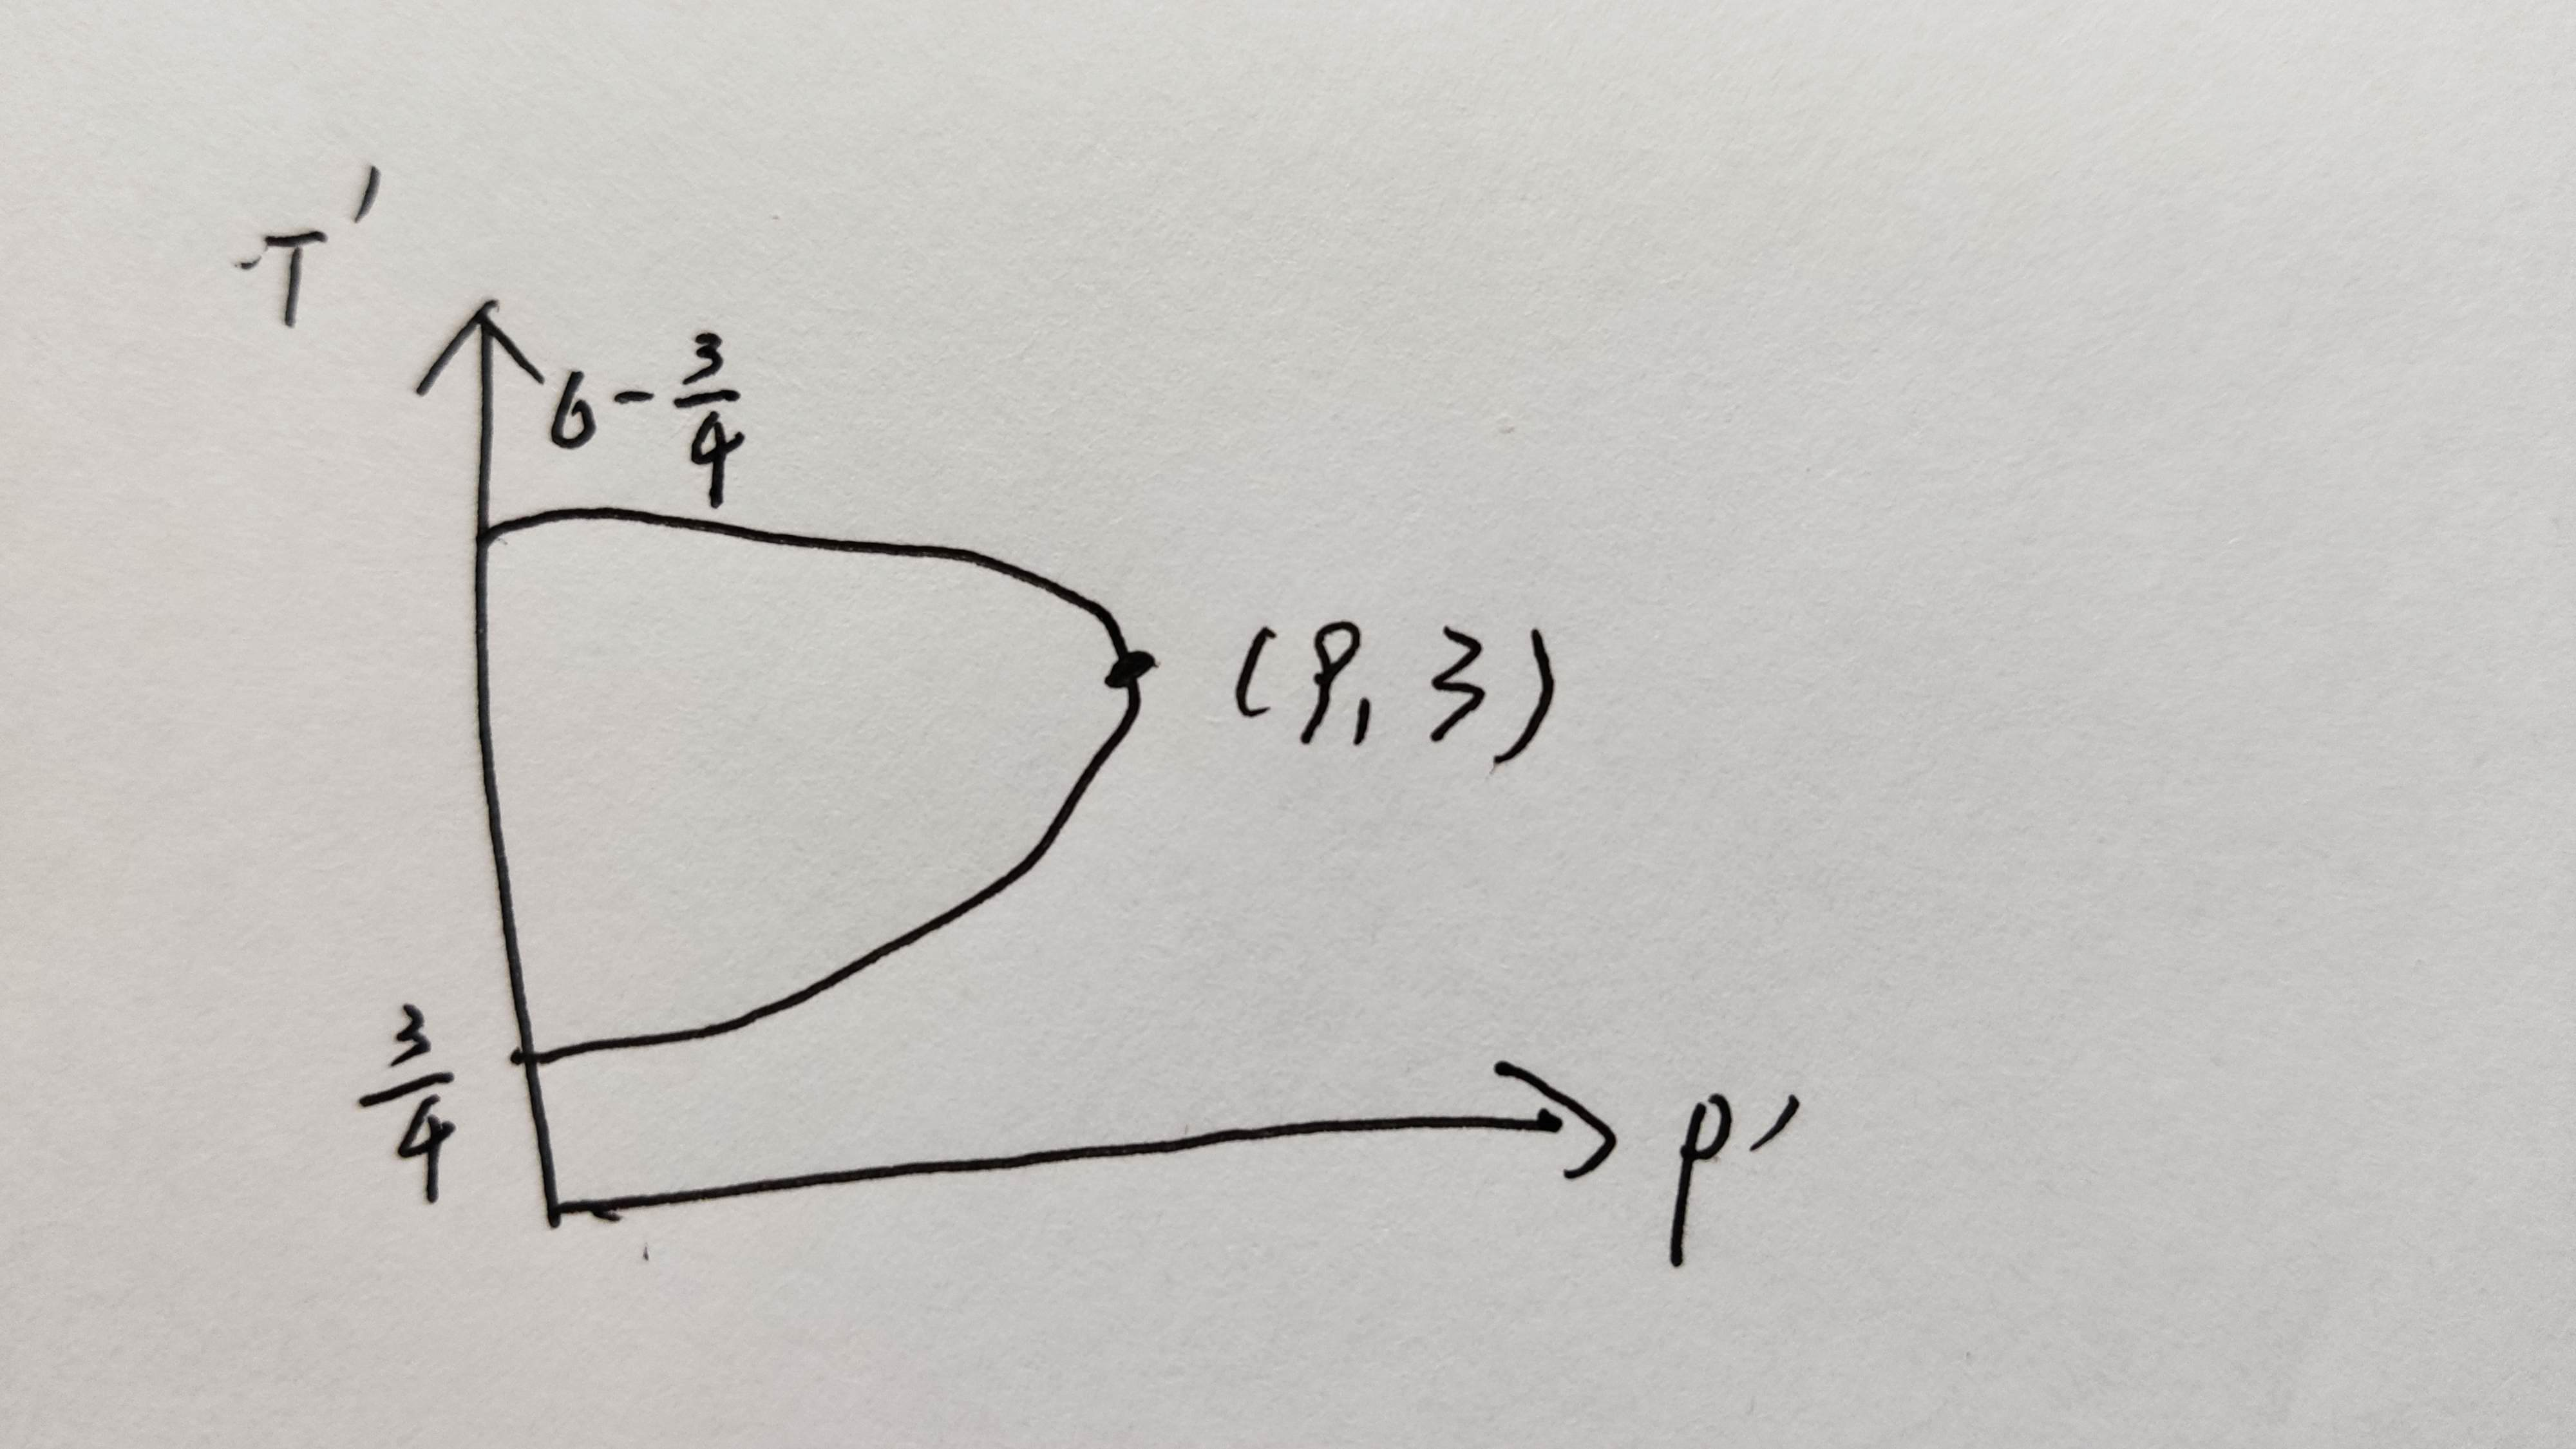
\includegraphics[width=90mm]{5.20Fig1.jpg}
        \caption{5.20 Figure 1}
    \end{figure}
    Problem 5.23\\
    Answer:\\
    (a)
    $$W=q_{1}-q_{2}=c\left(T_{1}-T_{f}\right)+c\left(T_{2}-T_{f}\right)=c\left(T_{1}+T_{2}-2 T_{f}\right) \eqno(8.1)$$
    (b)\\
    By the second law:
    $$\Delta S \geq 0 \eqno(8.2)$$
    Then:
    $$\int_{T_{1}}^{T_{f}} \frac{C d T}{T}+\int_{T_{2}}^{T_{f}} \frac{C d T}{T}=C \ln \frac{T_{f}^{2}}{T_{1}T_2} \geq 0 \eqno(8.3)$$
    So:
    $$T_{I}=\sqrt{T_1T_2} \eqno(8.4)$$
    (c)\\
    The maximum amount of work vill be obtained when $T_{f}=\sqrt{T_{1} T_{2}}$
    From (8.1):
    $$W=c\left(T_{1}+T_{2}-2 T_{f}\right)=C\left(\sqrt{T_{1}}-\sqrt{T}_{2}\right)^{2} \eqno(8.5)$$
    
    Problem 5.24\\
    Answer:\\
    To freeze an additional mass $m$ of water at $T_{0}$, heat $mL$ must be removed from the ice-water mixture resulting in an entrogy change $\Delta S_{1}=-\frac{mL}{\mathrm{T_0}}$.The heat rejected to the body of heat capacity $C$ increases its temperature to $T_{f}$ with an entropy change $\Delta S_{2}=C\int_{T_{0}}^{T_{f}} \frac{d T}{T}=C\,ln\frac{T_f}{T_{0}}$. By the second law $\Delta S_{1}+\Delta S_{2}=-\frac{m_{L}}{T_{0}}+C \ln \frac{T_{f}}{T_{0}} \geq 0 .$ For minimun temperature increase and thus ninimm heat rejection the equality holds and it follows that:
    $$T_{f}=T_{0} e^{\frac{mL}{T_0C}} \eqno(9.1)$$
    The heat rejected is $Q=C\left(T_{f}-T_{0}\right)=CT_{0}\left(e^{mL/T_{0} C}-1\right)$

    Problem 5.26\\
    Answer:\\
    In the processes $a \rightarrow b$ and $c \rightarrow d$ no heat is absorbed, so by the first law $W=-\Delta E$, and since $\Delta E=C\Delta T,$ where $C$ is the heat capacity, we have:
    $$W_{a \rightarrow b}=-\left(E_{b}-E_{a}\right)=-\nu c_{V}\left(T_{b}-T_{a}\right) \eqno(10.1)$$
    $$W_{c \rightarrow d}=-\left(E_{d}-E_{c}\right)=-\nu C_{V}\left(T_{d}-T_{c}\right) \eqno(10.2)$$
    Fovever, in an adiabatic expension $\mathrm{TV}^{\gamma-1}=$ const.\\
    Then:
    $$W_{a \rightarrow b}=-v c_{V} T_{b}\left(l \frac{T_{a}}{m_{b}}\right)=-v C_{V} T_{b}\left(1-\left(\frac{v_{2}}{v_{1}}\right)^{\gamma-1}\right)\eqno(10.3)$$
    $$W_{c \rightarrow d}=-v c_{V} T_{d}\left(l \frac{T_{d}}{m_{c}}\right)=-v C_{V} T_{c}\left(1-\left(\frac{v_{2}}{v_{1}}\right)^{\gamma-1}\right)\eqno(10.4)$$
    The volume is constant in process $b \rightarrow c$ so no work is performed.\\
    Then:
    $$Q_1=\left(E_{c}-E_{b}\right)=\nu C_{V}\left(T_{c}-T_{b}\right) \eqno(10.5)$$
    $$\eta=\frac{W_{a \rightarrow b}+W_{c \rightarrow d}}{Q_{1}}=l-\left(\frac{V_2}{V_{1}}\right)^{\gamma-1} \eqno(10.6)$$


\end{document}